\documentclass{article}

\title{Design notes for a distributed sorting application}
\author{Chengxin Ma}
\date{\today}

\usepackage[toc,page]{appendix}
\usepackage{graphicx}
\usepackage{hyperref}
\usepackage{todonotes}

\begin{document}

\maketitle

\section{Introduction}
This report describes the overall design of a distributed sorting application (Section \ref{sec:design}),
some key decisions in implementation (Section \ref{sec:implementation}), 
and a test run (including setup, result, and analysis) to see the performance of the application (Section \ref{sec:test_run}).
In addition, it contains the next steps of the work and predicted results (Section \ref{sec:todo}).

\section{Design}
\label{sec:design}
\subsection{Test data}
The final goal of designing this application is to integrate it into a genomic data process pipeline, where data in the SAM format
\footnote{\url{https://en.wikipedia.org/wiki/SAM_(file_format)\#Format}} is sorted.

From the perspective of sorting, the most interesting fields are \texttt{RNAME} (the name of the references sequence) and \texttt{POS} (position).
They together determine the order in which records are sorted.

Thus, to simplify the prototyping work, we design a data structure with three fields: \texttt{GROUP}, \texttt{SEQ}, and \texttt{DATA}.
Each record belongs to a group and has a sequence number in that group.
Its data is placed in the \texttt{DATA} field.

Here is an example input file: \href{https://github.com/MaChengxin/playground/blob/master/arrow/flight/my_flight/data/4_nodes/records_on_node_0.txt}{\textit{Input records on Node 0}},
and here is an example file containing expected sorted records: \href{https://github.com/MaChengxin/playground/blob/master/arrow/flight/my_flight/data/4_nodes/expected_records_on_node_0.txt}{\textit{Expected sorted records on Node 0}}.
Note that we do not necessarily need to write the output into files.
It is only for experimenting purpose.
After integration we could use in-memory storage instead.

\subsection{Functional decomposition and phases}

The following functional components must be implemented to complete the application.
\begin{itemize}
    \item sorter
    \item sender and receiver
    \item partitioner and merger
    \item storage (optional)
\end{itemize}

The \textit{sorter} is responsible for sorting the data in our desired order: records with smaller Group IDs are placed before those with large Group IDs.
If the Group IDs of two records are the same, the secondary criteria is the sequence number.

The \textit{sender} and \textit{receiver} are responsible for sending data to destination nodes and receiving data from source node respectively.

The responsibility of the \textit{partitioner} is to partition the data into different groups that would be sent to different destinations,
while the \textit{merger} is to merge the partitioned data to a complete set.

\textit{Storage} is needed when we want to temporarily store the data before further processing.

Based on if data is shuffled or not during execution, we can divide the overall execution time into three phases.

The first phase is the \textit{partitioning} phase.
In this phase, data is partitioned to subsets according to the final destination where it is going to be sent to.
Beginning of this phase is marked by the earliest start time on all the nodes,
while the end of this phase is marked by the time when all nodes have finished partitioning and serializing the input data.

The second phase is the \textit{communication} phase.
In this phase, data is shuffled to destination nodes in parallel.
As soon as one node has started sending data out, it is the time that marks the beginning of the communication phase.
End of this phase is marked by the time when all nodes have received all data belonging to them.

The third phase is the \textit{sorting} phase.
In this phase, data from all other nodes and on the local node is merged and sorted.
Beginning and end of this phase is marked by the earliest start time of deserialization on all nodes and the latest finish time of sorting on all nodes respectively.

\section{Implementation}
\label{sec:implementation}

\subsection{Implementation choices}
We choose \texttt{pandas}, a Python library for data manipulation and analysis, 
for the partitioning and sorting phase of the application.
For the communication phase, we have two alternatives: Python's \texttt{socket} module and \texttt{Apache Arrow Flight}.
The interface to the partitioning phase and sorting phase is thus also different.
We use \texttt{pickle} to serialize/deserialize the data before/after the communication phase in the \texttt{socket} approach,
while \texttt{Plasma} and \texttt{Arrow RecordBatch} are used when we use \texttt{Apache Arrow Flight} for communication.

To achieve parallelism in communication, in the \texttt{socket} approach, we use the \texttt{multiprocessing} module 
(instead of \texttt{threading} which cannot take advantage of multiple cores due to the existence of \texttt{CPython}'s Global Interpreter Lock),
while for the \texttt{Apache Arrow Flight} approach we use \texttt{Arrow}'s internal \texttt{ThreadPool}.
\todo[]{Can experiment result show if they are correctly implemented?}

\subsection{Flowchart}

Figure \ref{fig:flowchart} shows the overall flowchart of the distributed sorting application.


\begin{figure}[h!]
    \centering
    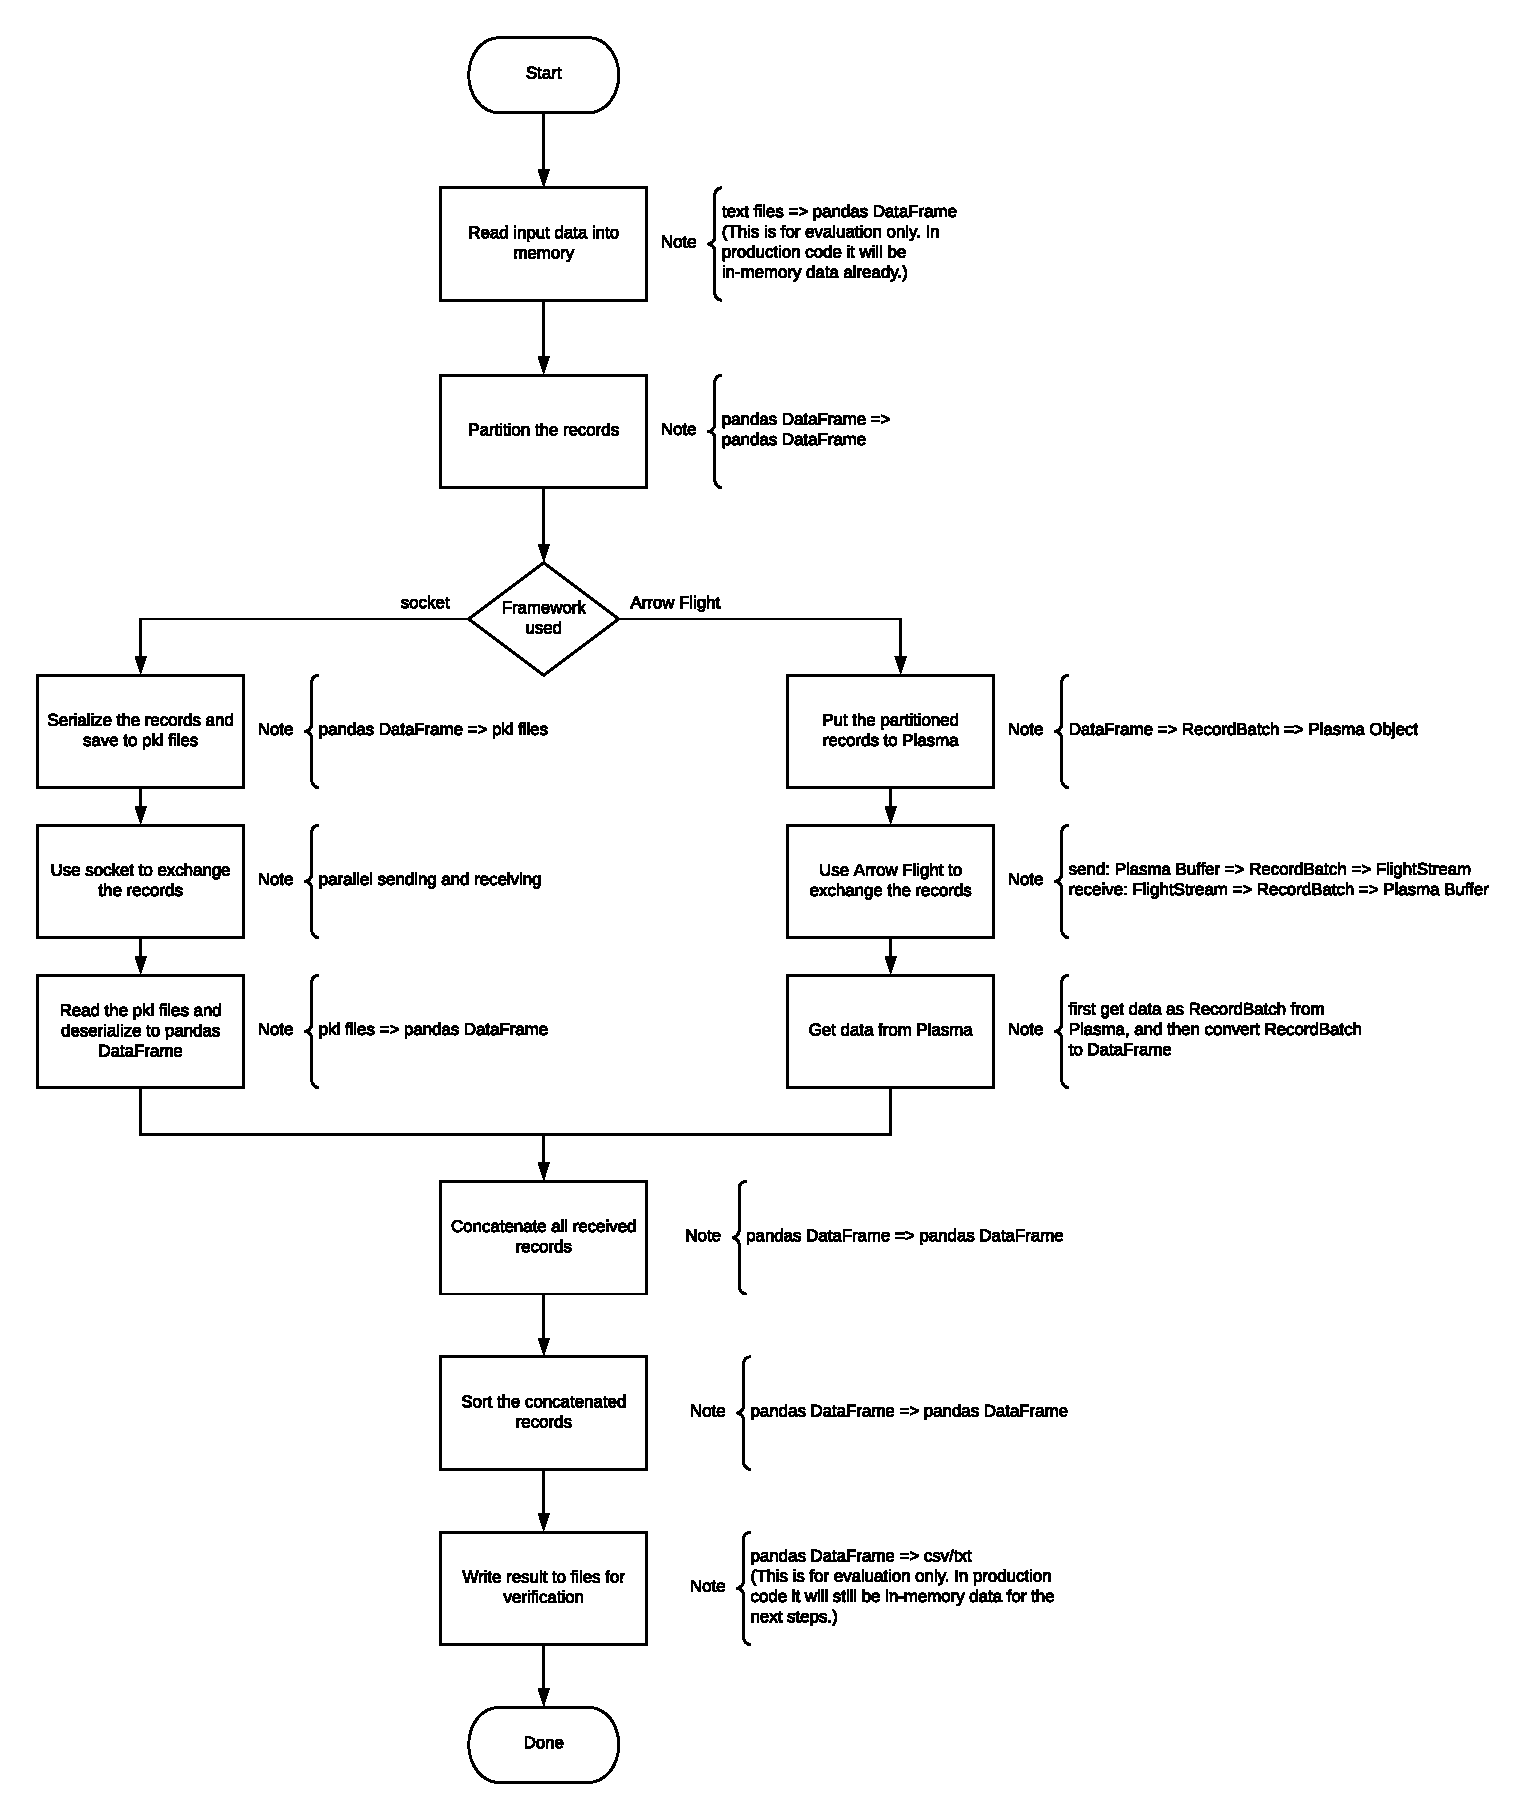
\includegraphics[width=1.2\textwidth]{flowchart}
    \caption{Flowchart of the application, with two alternatives for the communication phase}
    \label{fig:flowchart}
\end{figure}

\section{Test run}
\label{sec:test_run}

\subsection{Setup}
To see the performance of the application, a test run has been performed.
4 nodes on Cartesius (\texttt{tcn798, tcn799, tcn804, tcn807}, we refer them as from Node 0 to 3 hereafter) were allocated for this test run.
The data for the test run contains records of 40 groups (from \texttt{GROUP0} to \texttt{GROUP39}), each having 2 million records (i.e. the total number of records is 80 million).
Each node had 20 million records in random order before the application ran, and we expected that when the application finishes,
Node 0 stores records from \texttt{GROUP0} to \texttt{GROUP9},
Node 1 stores records from \texttt{GROUP10} to \texttt{GROUP19},
Node 2 stores records from \texttt{GROUP20} to \texttt{GROUP29},and
Node 3 stores records from \texttt{GROUP30} to \texttt{GROUP39}, in the ascending order.

The size of the input and output files on each node is around 540 MB.

The test run was started one by one manually, in the order of from Node 0 to 3.

\subsection{Results}
The tables in Appendix \ref{appendix:test_run_results} show the original timestamp of tasks on these four nodes.

To have a more straightforward view, we have adjusted the original timestamp by setting the starting time to 0:00:00.

\begin{table}[h!]
  \begin{tabular}{|l|l|l|l|l|}
  \hline
                                                & \textbf{tcn798} & \textbf{tcn799} & \textbf{tcn804} & \textbf{tcn807} \\ \hline
  started partitioning the records              & 0:00:00         & 0:00:00         & 0:00:00         & 0:00:02         \\ \hline
  \begin{tabular}[c]{@{}l@{}}finished partitioning the records, \\ started serializing the data to pkl files\end{tabular}     & 0:00:15 & 0:00:14 & 0:00:15 & 0:00:18 \\ \hline
  \begin{tabular}[c]{@{}l@{}}finished serializing the data to pkl files, \\ started sending to destination nodes\end{tabular} & 0:00:29 & 0:00:26 & 0:00:29 & 0:00:33 \\ \hline
  received last file                            & 0:00:35         & 0:00:35         & 0:00:35         & 0:00:35         \\ \hline
  started unpickling the records from pkl files & 0:00:36         & 0:00:36         & 0:00:36         & 0:00:36         \\ \hline
  \begin{tabular}[c]{@{}l@{}}finished unpickling the records from pkl files, \\ started concatenating\end{tabular}            & 0:00:39 & 0:00:39 & 0:00:39 & 0:00:39 \\ \hline
  \begin{tabular}[c]{@{}l@{}}finished concatenating, \\ started sorting the records\end{tabular}                              & 0:00:43 & 0:00:43 & 0:00:43 & 0:00:43 \\ \hline
  finished sorting the records                  & 0:00:58         & 0:00:59         & 0:00:58         & 0:00:59         \\ \hline
  \end{tabular}
  \caption{Adjusted timestamp of the distributed sorting application (using socket) on 4 nodes}
  \label{tab:adj-time-socket}
\end{table}

\begin{table}[h!]
  \begin{tabular}{|l|l|l|l|l|}
  \hline
                                                      & \textbf{tcn798} & \textbf{tcn799} & \textbf{tcn804} & \textbf{tcn807} \\ \hline
  started partitioning the records                    & 0:00:01         & 0:00:01         & 0:00:00         & 0:00:00         \\ \hline
  \begin{tabular}[c]{@{}l@{}}finished partitioning the records, \\ started putting them to Plasma\end{tabular}            & 0:00:16 & 0:00:20 & 0:00:15 & 0:00:15 \\ \hline
  finished putting partitioned records to Plasma      & 0:00:21         & 0:00:23         & 0:00:18         & 0:00:19         \\ \hline
  send-to-dest started                                & 0:00:23         & 0:00:26         & 0:00:20         & 0:00:22         \\ \hline
  received last piece of data                         & 0:00:26         & 0:00:26         & 0:00:26         & 0:00:26         \\ \hline
  started retrieving the records from Plasma          & 0:00:27         & 0:00:27         & 0:00:27         & 0:00:27         \\ \hline
  \begin{tabular}[c]{@{}l@{}}finished retrieving the records from Plasma, \\ started converting to DataFrame\end{tabular} & 0:00:27 & 0:00:27 & 0:00:27 & 0:00:27 \\ \hline
  \begin{tabular}[c]{@{}l@{}}finished converting to DataFrame, \\ started concatenating\end{tabular}                      & 0:00:35 & 0:00:35 & 0:00:35 & 0:00:35 \\ \hline
  finished concatenating, started sorting the records & 0:00:38         & 0:00:37         & 0:00:37         & 0:00:38         \\ \hline
  finished sorting the records                        & 0:00:53         & 0:00:52         & 0:00:52         & 0:00:53         \\ \hline
  \end{tabular}
  \caption{Adjusted timestamp of the distributed sorting application (using Apache Arrow Flight) on 4 nodes}
  \label{tab:adj-time-flight}
\end{table}

As can be seen in Table \ref{tab:adj-time-socket} and \ref{tab:adj-time-flight},
both implementations can complete the tasks with in 1 minute.
The \texttt{Flight} implementation (53 seconds) is 6 seconds faster than the \texttt{socket} implementation (59 seconds).

\subsection{Discussion: Where does the difference come from?}

The difference comes from (de)serialization and communication.
In the \texttt{socket} approach, serializing \texttt{DataFrame} to \texttt{pickle} files took 13.75 seconds on average,
while in the \texttt{Flight} approach, putting partitioned \texttt{DataFrame} to \texttt{Plasma} only took 3.75 second on average.
Unpickling \texttt{pickle} files to \texttt{DataFrame} took 3 seconds, while converting data from \texttt{Plasma} to \texttt{DataFrame} took 8 seconds.
Therefore, using \texttt{Arrow} saves us 5 seconds in (de)serialization from using \texttt{socket}.

The above average time of (de)serialization was calculated by $\frac{1}{4}\sum_{i=0}^{3} (finish\_time_i - start\_time_i)$.
We cannot apply the same formula for calculating communication time, since for one sending from one node there are multiple receiving on multiple nodes.
We thus use the following formula to calculate the communication time: $\frac{1}{4}\sum_{i=0}^{3} (max(finish\_time_{ij}) - start\_time_{i})$,
where $finish\_time_{ij}$ denotes the time when node $j$ finished receiving from node $i$.

In the \texttt{socket} implementation, these four nodes sent out data at \texttt{13:08:15}, \texttt{13:08:18}, \texttt{13:08:18}, and \texttt{13:08:22}.
The receiver logs (see Figure \ref{fig:tcn799_r_log_socket} as an example) show that these nodes received first batch of files at \texttt{13:08:16}, \texttt{13:08:17}, 
or \texttt{13:08:18}, the second and third batch of files at \texttt{13:08:22}, and the last batch at \texttt{13:08:24}.
The average communication time is thus 3.25 seconds.
We also noticed that sending the second and third batches started at the same time, and receiving them finished at the same time as well.
These two fully overlapped communication took 4 seconds, which is the longest communication time we have observed.
This might be a sign that at this point the application is already IO bounded and multiprocessing won't help much in acceleration.

For the \texttt{Flight} implementation, after examining the logs (see Figure \ref{fig:tcn798_r_log_flight} as an example) of these nodes, 
we found that as soon as one node sent out the data, all nodes (including the sender itself) would receive it immediately.
Since the granularity of logging is 1 second, we assume that communication is 0.5 second.

Based on the analysis above, we estimate that using \texttt{Arrow Flight} saves approximately 3 seconds than using \texttt{socket} for communication.

\subsection{Discussion: How much does each task take up in the overall execution?}

It is also important to see how much time each task take in the overall execution,
such that we can determine the direction for optimization.

We have plotted two pie charts of the amount of time each task took in the \texttt{socket} approach and in the \texttt{Flight} approach.
(We used the C++ version of \texttt{Arrow Flight} and we noticed that there is a "switch time" from Python to C++.
See Appendix \ref{appendix:known_issues} for more details.)


\begin{figure}[h!]
  \centering
  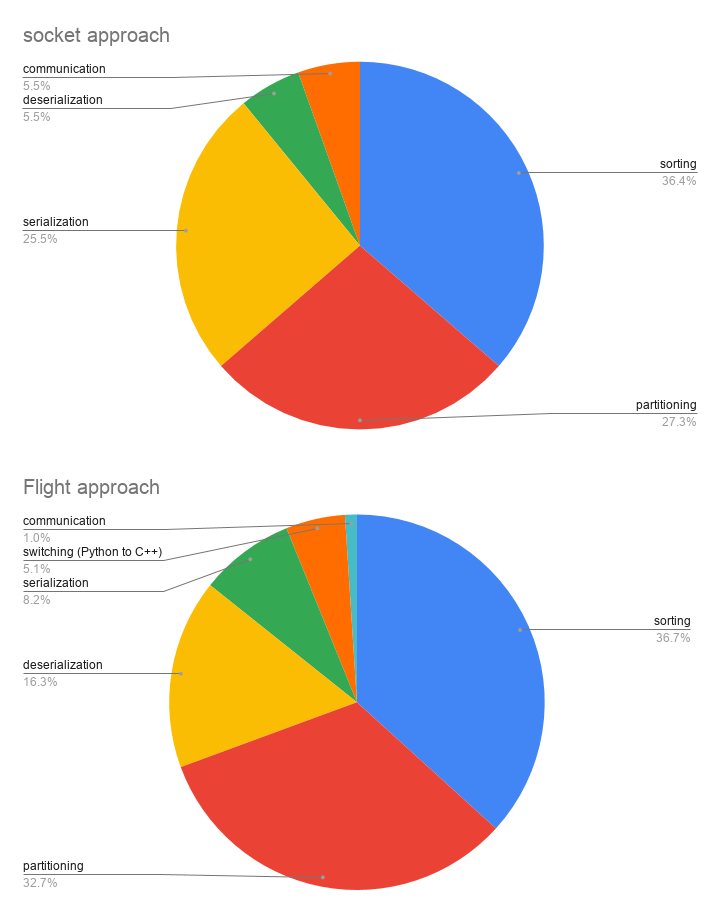
\includegraphics[width=0.75\textwidth]{pie_chart_socket_vs_flight}
  \caption{Comparison of the percentage each task took in two approaches}
  \label{fig:pie_chart_socket_vs_flight}
\end{figure}

We see that most of the time was spent on partitioning, sorting, adn SerDes.
The communication phase does not take up much time in both cases.

\subsection{Discussion: Load balancing}

So far, load balancing looks good.
See Figure \ref{fig:timestamp_socket_vs_flight} for a visualized result.

\begin{figure}[h!]
  \centering
  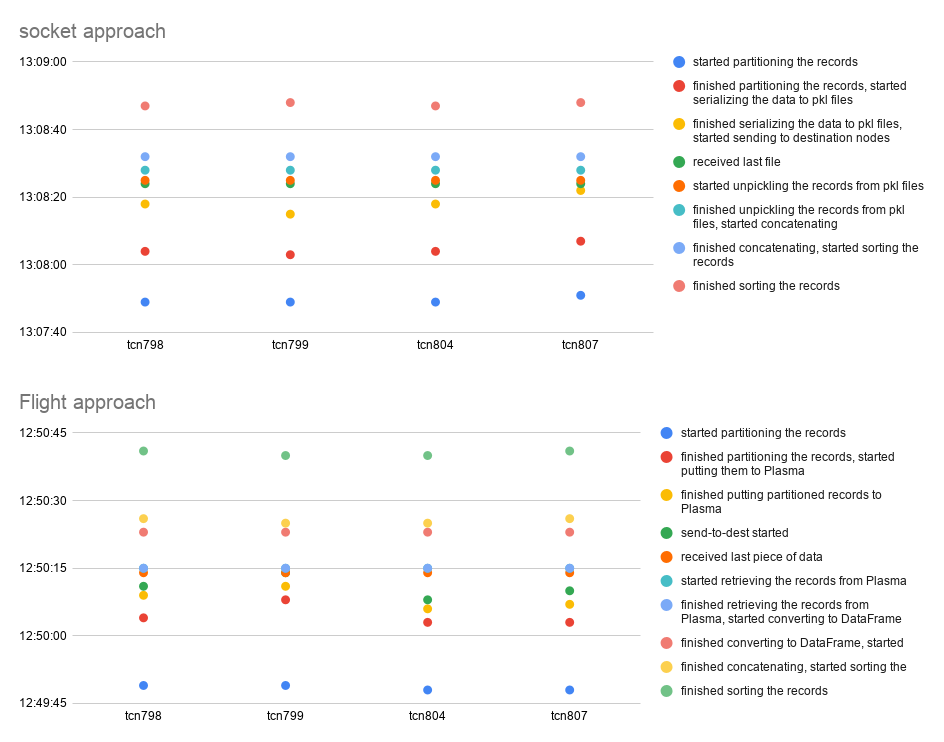
\includegraphics[width=1.0\textwidth]{timestamp_socket_vs_flight}
  \caption{Timestamp of tasks in two approaches}
  \label{fig:timestamp_socket_vs_flight}
\end{figure}


\section{Running in a larger scale}
\label{sec:todo}
\textbf{\textit{This part still in progress. Here is my predication.}}

If we use more nodes and more data to perform distributed sorting,
does the conclusions we made in Section \ref{sec:test_run} still hold?

We expect that:
\begin{itemize}
  \item in both approaches (\texttt{socket} and \texttt{Flight}), the percentage of time spent on partitioning and sorting would decrease;
  \item in both approaches, the percentage of time spent on communication would increase;
  \item the time save by using \texttt{Arrow} and \texttt{Flight} instead of \texttt{pickle} and \texttt{socket} would increase. 
\end{itemize}

\newpage
\begin{appendices}

\section{Test run results}
\label{appendix:test_run_results}

See Table \ref{tab:orig-time-socket} and \ref{tab:orig-time-flight} for the original timestamp of the distributed sorting application.

\begin{table}[h!]
  \begin{tabular}{|l|l|l|l|l|}
  \hline
                                                & \textbf{tcn798} & \textbf{tcn799} & \textbf{tcn804} & \textbf{tcn807} \\ \hline
  started partitioning the records              & 13:07:49        & 13:07:49        & 13:07:49        & 13:07:51        \\ \hline
  \begin{tabular}[c]{@{}l@{}}finished partitioning the records, \\ started serializing the data to pkl files\end{tabular}     & 13:08:04 & 13:08:03 & 13:08:04 & 13:08:07 \\ \hline
  \begin{tabular}[c]{@{}l@{}}finished serializing the data to pkl files, \\ started sending to destination nodes\end{tabular} & 13:08:18 & 13:08:15 & 13:08:18 & 13:08:22 \\ \hline
  received last file                            & 13:08:24        & 13:08:24        & 13:08:24        & 13:08:24        \\ \hline
  started unpickling the records from pkl files & 13:08:25        & 13:08:25        & 13:08:25        & 13:08:25        \\ \hline
  \begin{tabular}[c]{@{}l@{}}finished unpickling the records from pkl files, \\ started concatenating\end{tabular}            & 13:08:28 & 13:08:28 & 13:08:28 & 13:08:28 \\ \hline
  \begin{tabular}[c]{@{}l@{}}finished concatenating, \\ started sorting the records\end{tabular}                              & 13:08:32 & 13:08:32 & 13:08:32 & 13:08:32 \\ \hline
  finished sorting the records                  & 13:08:47        & 13:08:48        & 13:08:47        & 13:08:48        \\ \hline
  \end{tabular}
  \caption{Original timestamp of the distributed sorting application (using socket) on 4 nodes}
  \label{tab:orig-time-socket}
\end{table}

\begin{table}[h!]
  \begin{tabular}{|l|l|l|l|l|}
  \hline
                                                 & \textbf{tcn798} & \textbf{tcn799} & \textbf{tcn804} & \textbf{tcn807} \\ \hline
  started partitioning the records               & 12:49:49        & 12:49:49        & 12:49:48        & 12:49:48        \\ \hline
  \begin{tabular}[c]{@{}l@{}}finished partitioning the records, \\ started putting them to Plasma\end{tabular}            & 12:50:04 & 12:50:08 & 12:50:03 & 12:50:03 \\ \hline
  finished putting partitioned records to Plasma & 12:50:09        & 12:50:11        & 12:50:06        & 12:50:07        \\ \hline
  send-to-dest started                           & 12:50:11        & 12:50:14        & 12:50:08        & 12:50:10        \\ \hline
  received last piece of data                    & 12:50:14        & 12:50:14        & 12:50:14        & 12:50:14        \\ \hline
  started retrieving the records from Plasma     & 12:50:15        & 12:50:15        & 12:50:15        & 12:50:15        \\ \hline
  \begin{tabular}[c]{@{}l@{}}finished retrieving the records from Plasma, \\ started converting to DataFrame\end{tabular} & 12:50:15 & 12:50:15 & 12:50:15 & 12:50:15 \\ \hline
  \begin{tabular}[c]{@{}l@{}}finished converting to DataFrame, \\ started concatenating\end{tabular}                      & 12:50:23 & 12:50:23 & 12:50:23 & 12:50:23 \\ \hline
  \begin{tabular}[c]{@{}l@{}}finished concatenating, \\ started sorting the records\end{tabular}                          & 12:50:26 & 12:50:25 & 12:50:25 & 12:50:26 \\ \hline
  finished sorting the records                   & 12:50:41        & 12:50:40        & 12:50:40        & 12:50:41        \\ \hline
  \end{tabular}
  \caption{Original timestamp of the distributed sorting application (using Apache Arrow Flight) on 4 nodes}
  \label{tab:orig-time-flight}
\end{table}

\begin{figure}[h!]
  \centering
  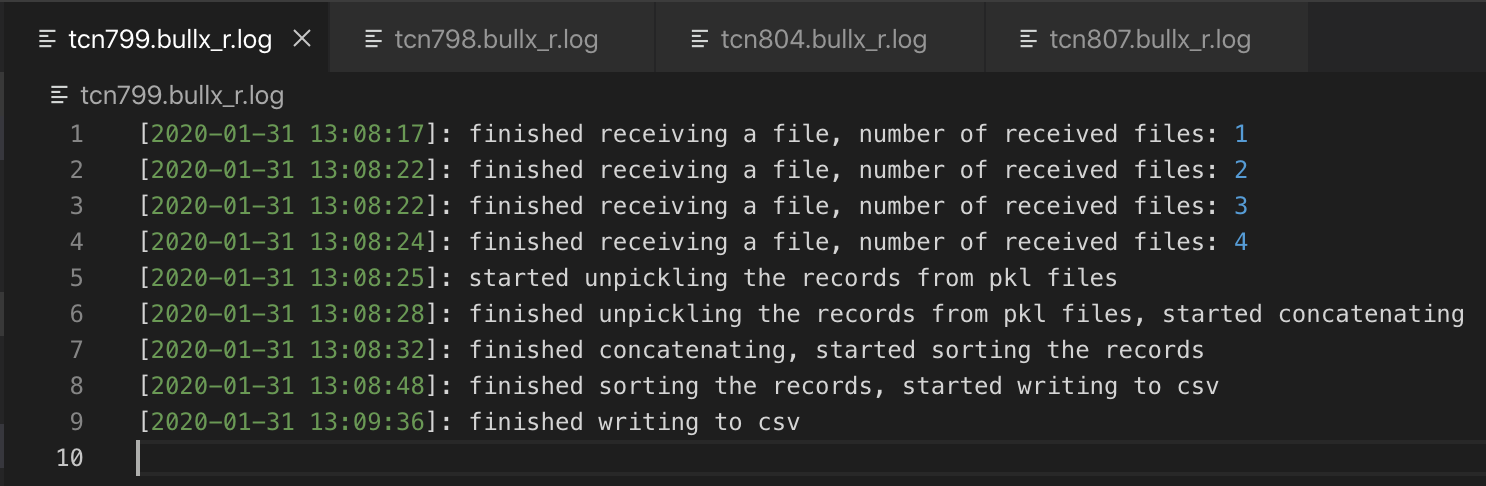
\includegraphics[width=1.0\textwidth]{tcn799_r_log_socket}
  \caption{log (receiver part) of node \texttt{tcn799}, socket approach}
  \label{fig:tcn799_r_log_socket}
\end{figure}

\begin{figure}[h!]
  \centering
  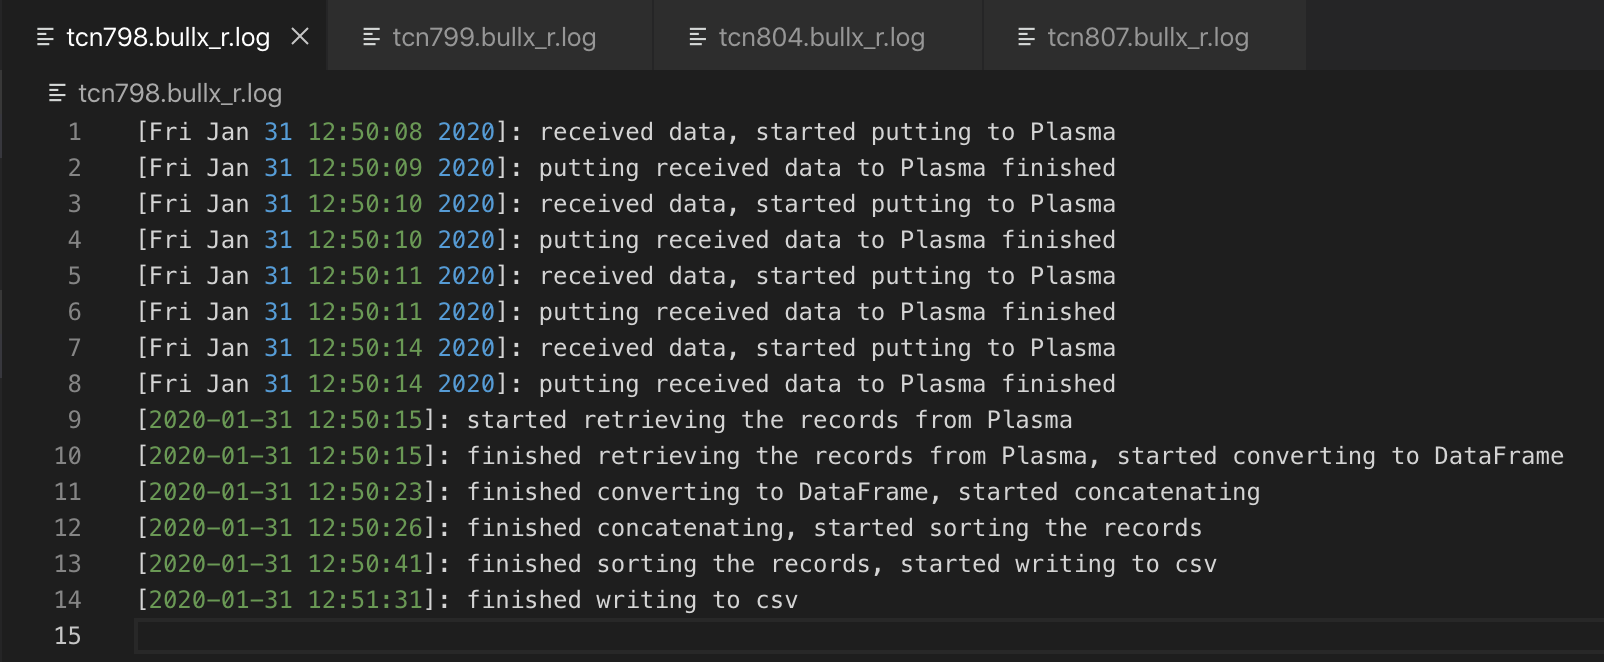
\includegraphics[width=1.0\textwidth]{tcn798_r_log_flight}
  \caption{log (receiver part) of node \texttt{tcn798}, Flight approach}
  \label{fig:tcn798_r_log_flight}
\end{figure}

\section{Known issues}
\label{appendix:known_issues}

\subsection{Building the project}

On macOS, the \texttt{grpc} library installed via \texttt{Homebrew} (as a dependency of \texttt{apache-arrow}) seems to be problematic.
The Flight server would incur a segmentation fault due to the current version (stable 1.26.0) of \texttt{grpc}.

We can make use of the existing build system of arrow to build \texttt{grpc} from source.
(The build system is capable of building any missing dependency from source.)
This also saves us from building missing dependencies manually on Cartesius.

\subsection{Switch time}
Since we used the C++ implementation of \texttt{Arrow Flight}, we need to switch from the Python process performing the partitioning task
after it is done.
The time used for switching from the Python process to C++ process is around 3 seconds, which is more than expected.
Since our concern is computation (including partitioning, sorting, and SerDes) and communication, we ignore this issue for now.
For analysis we can simply remove this part from the total execution time.

\end{appendices}

\end{document}
